\subsection{Aplicação}

Para a aplicação em questão, é determinado o intervalo de confiança onde um nível de confiança de $95\%$ foi considerado.

\begin{figure}[H]
	\centering
	\caption{Intervalo de Confiança para a Força Axial} 
	{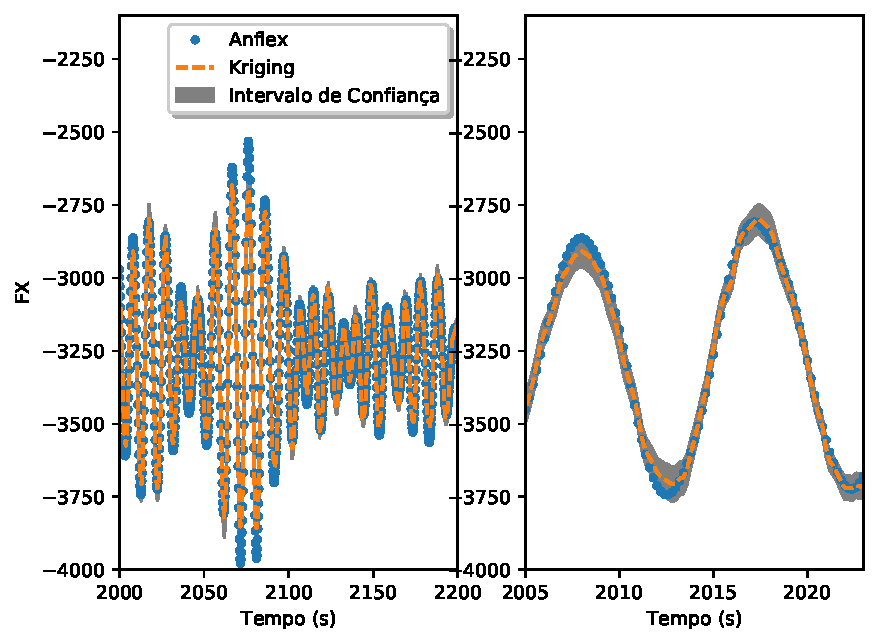
\includegraphics[width=0.7\linewidth]{tatiane/fig_tati/ic/ic_riser1.pdf}} 
	\flushleft \footnotesize{Fonte: Elaborada pela autora.} 
	\label{fig:ic2}
\end{figure}

Na Figura (\ref{fig:ic2}), observa-se que o intervalo de confiança considerado contém a resposta simulada via Anflex para a Força Axial e, que em alguns locais a resposta está próxima das extremidades do intervalo de confiança. 

Destaca-se que o Kriging retorna a média e variância de um processo gaussiano, uma possibilidade para melhorar o metamodelo adicionando novos pontos em regiões onde a área do intervalo de confiança é larga.